\scanpage{61}
% His upper-right number; only the lower, open oval frame survives at the clipped top edge.
\mspage{\makebox[0pt][l]{\begin{tikzpicture}[overlay,baseline=0pt]
\draw (-.22,.15) .. controls (-.24,-.22) and (.55,-.22) .. (.54,.15);
\end{tikzpicture}}18}
avec $k$ successeur de $i$, il s'agit de singularité isolée, mais dans le cas de $\mathcal{V}_{i,k}^k$ général, on peut trouver des singularités de type arbitraire bien sûr en fibre (prendre $X_i=X_i^*$ réduit à un pt !) — ce qui diminue l'intérêt, dans le cas de stratifications tant soit peu générales, des $\mathcal{V}_{i,k}^j$ généraux comme ``pierres''. Les $\mathcal{V}_{i,k}^{j}=\mathcal{V}_{i,k}^*$ sont déjà plus intéressants, car \deleted{\unsure{ce sont}} c'est essentiellement un \inserted{germe d'} ouvert de $X_k^*$, donc non singulier — ce qui \unsure{s'exprimera|s'exprime} par le fait qu'on l'obtient comme un fibré sur $X_i^*$ non singulier, à fibre non singulière $\mathcal{V}_{\unsure{z|Z},Z_{i,k}}^*$ \ldots

Donc nous allons dans la suite systématiquement essayer d'exprimer le maximum avec les $X_i^*$ et \inserted{les} $\mathcal{V}_{i,j}$, $\mathcal{V}_{i,j}^*$ ``élémentaires'' ($j$ successeur de $i$), puis voir si certaines expressions peuvent prendre une forme plus sympathique en utilisant aussi \inserted{les $X_i^*$ et} les $\mathcal{V}_{\unsure{i,j|ijj}}$, $\mathcal{V}_{i,j}^*$ avec $i\leq j$ \unsure{sans|dans} plus — et dans un dernier temps seulement, peut-être (\unsure{en|eu} égard au cas des diviseurs \unsure{à|:} croisements normaux) voir comment les $\mathcal{V}_{i,k}^j$ s'insèrent dans ce formalisme.
% Pale lower-left foliation, another hand.
\margin{60}
